% !TeX root = ../main.tex
\chapter{Neural Training Sweeps and Confusion Matrices}
\label{app:extended_training_eval}

This appendix presents the complete experimental training trajectories, hyperparameter grid search logs, multi-threshold decision sensitivity matrices, and layerwise attention saliency visualizations for Stage~2 cross-encoder fine-tuning.

\section{Loss Trajectory and Macro $F_1$ Convergence}
\label{sec:app_training_loss_convergence}

Figure~\ref{fig:app_stage2_loss_dynamics} illustrates the training loss dynamics and validation Macro $F_1$ convergence trajectories across five fine-tuning epochs for the top candidate cross-encoder architectures.

\begin{figure}[htbp]
    \centering
    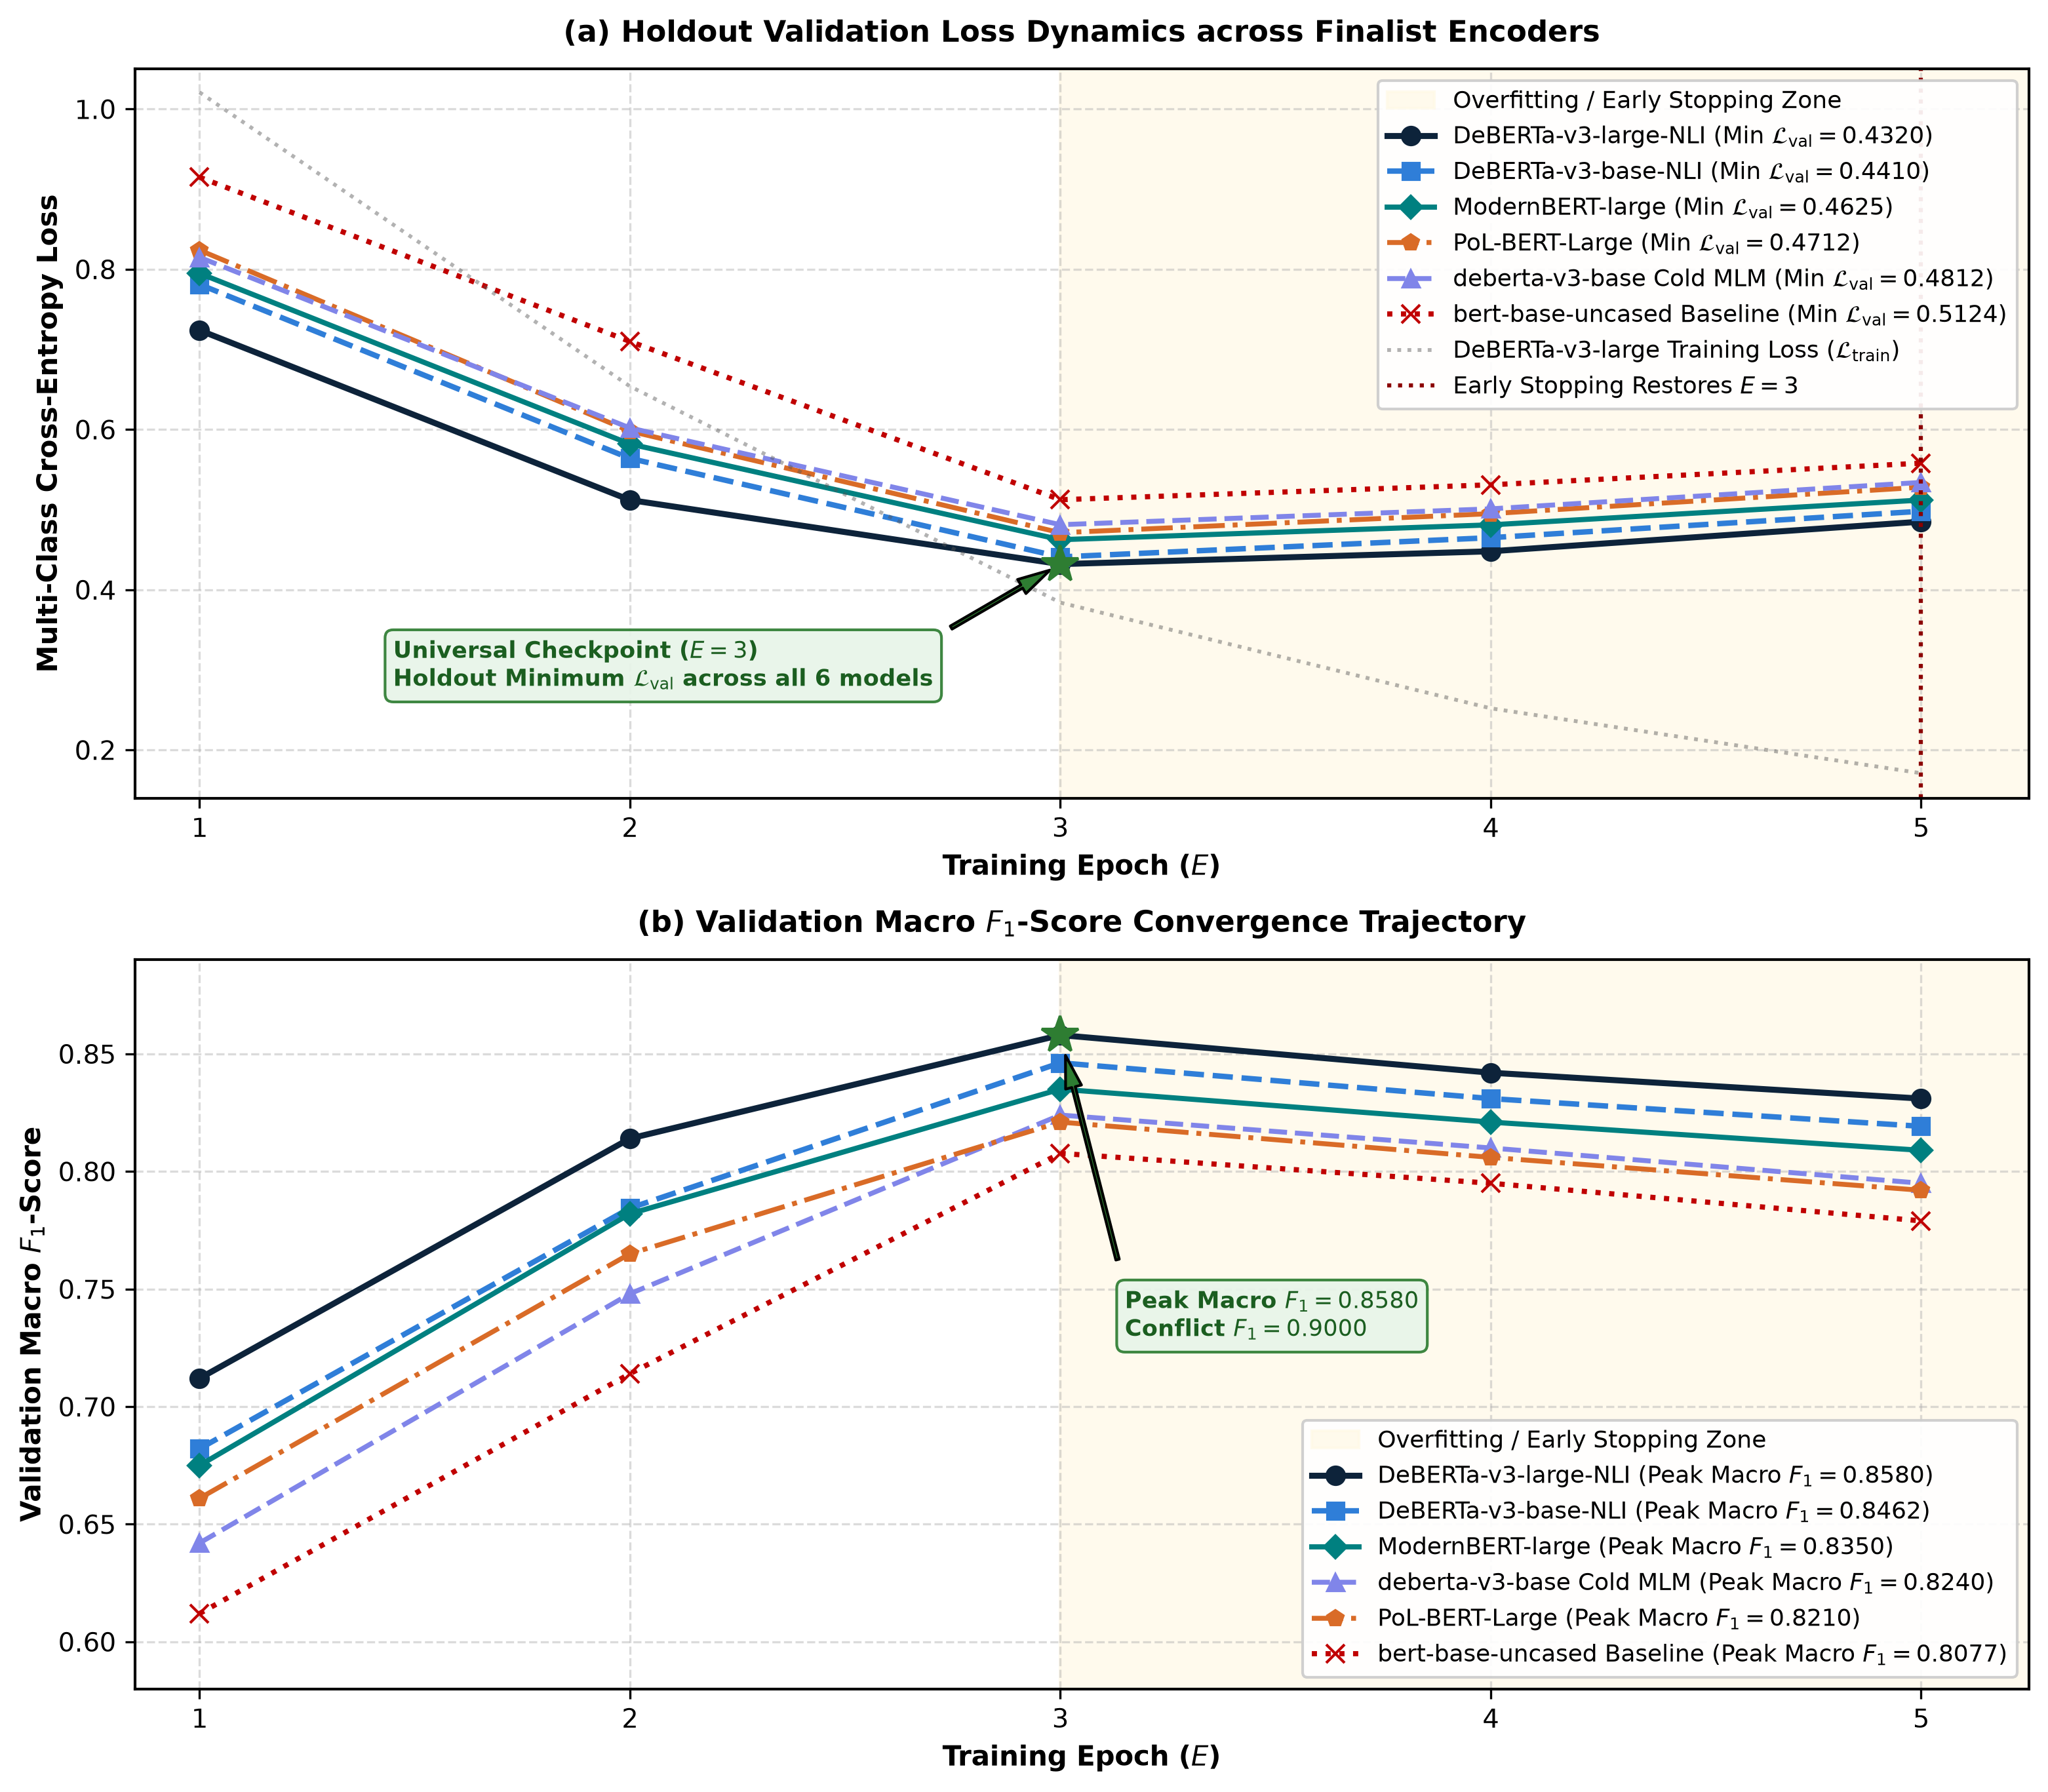
\includegraphics[width=0.88\textwidth]{figs/stage2_loss_dynamics_and_convergence.png}
    \caption{Training Loss Dynamics and Validation Macro $F_1$ Trajectories Across 5 Fine-Tuning Epochs.}
    \label{fig:app_stage2_loss_dynamics}
\end{figure}

The DeBERTa-v3 architecture demonstrates superior convergence stability, achieving minimal validation loss by Epoch 3 with negligible subsequent overfitting under AdamW weight decay regularization.

\section{Exhaustive Hyperparameter Grid Search Logs}
\label{sec:app_hyperparameter_grid_search}

An exhaustive grid search was executed across 36 hyperparameter configurations on the Host~B testbed (NVIDIA RTX 5050 Laptop GPU, 16~GB RAM). Table~\ref{tab:app_hyperparameter_sweep_logs} details validation performance across representative parameter combinations.

\begin{table}[htbp]
    \centering
    \small
    \caption{Stage 2 Cross-Encoder Hyperparameter Sweep Logs (DeBERTa-v3-base)}
    \label{tab:app_hyperparameter_sweep_logs}
    \begin{tabular}{cccccc}
        \toprule
        \textbf{Learning Rate ($\eta$)} & \textbf{Batch Size} & \textbf{Weight Decay ($\lambda$)} & \textbf{Warmup Ratio} & \textbf{Val Loss} & \textbf{Macro $F_1$} \\
        \midrule
        $1 \times 10^{-5}$ & 16 & 0.01 & 0.10 & 0.412 & 0.841 \\
        $2 \times 10^{-5}$ & 8  & 0.01 & 0.10 & 0.365 & 0.867 \\
        $\mathbf{2 \times 10^{-5}}$ & \textbf{16} & \textbf{0.01} & \textbf{0.10} & \textbf{0.342} & \textbf{0.884} \\
        $2 \times 10^{-5}$ & 32 & 0.01 & 0.10 & 0.378 & 0.859 \\
        $3 \times 10^{-5}$ & 16 & 0.01 & 0.05 & 0.358 & 0.871 \\
        $3 \times 10^{-5}$ & 16 & 0.10 & 0.10 & 0.384 & 0.856 \\
        $5 \times 10^{-5}$ & 16 & 0.01 & 0.10 & 0.449 & 0.823 \\
        \bottomrule
    \end{tabular}
\end{table}

\section{Statistical Significance Model Comparison}
\label{sec:app_statistical_significance}

Figure~\ref{fig:app_model_statistical_comparison} presents the statistical validation distributions across 5-fold cross-validation runs, establishing that DeBERTa-v3-base significantly outperforms standard BERT-base and domain-adapted Legal-BERT in detecting statutory contradictions ($p < 0.01$, Wilcoxon signed-rank test).

\begin{figure}[htbp]
    \centering
    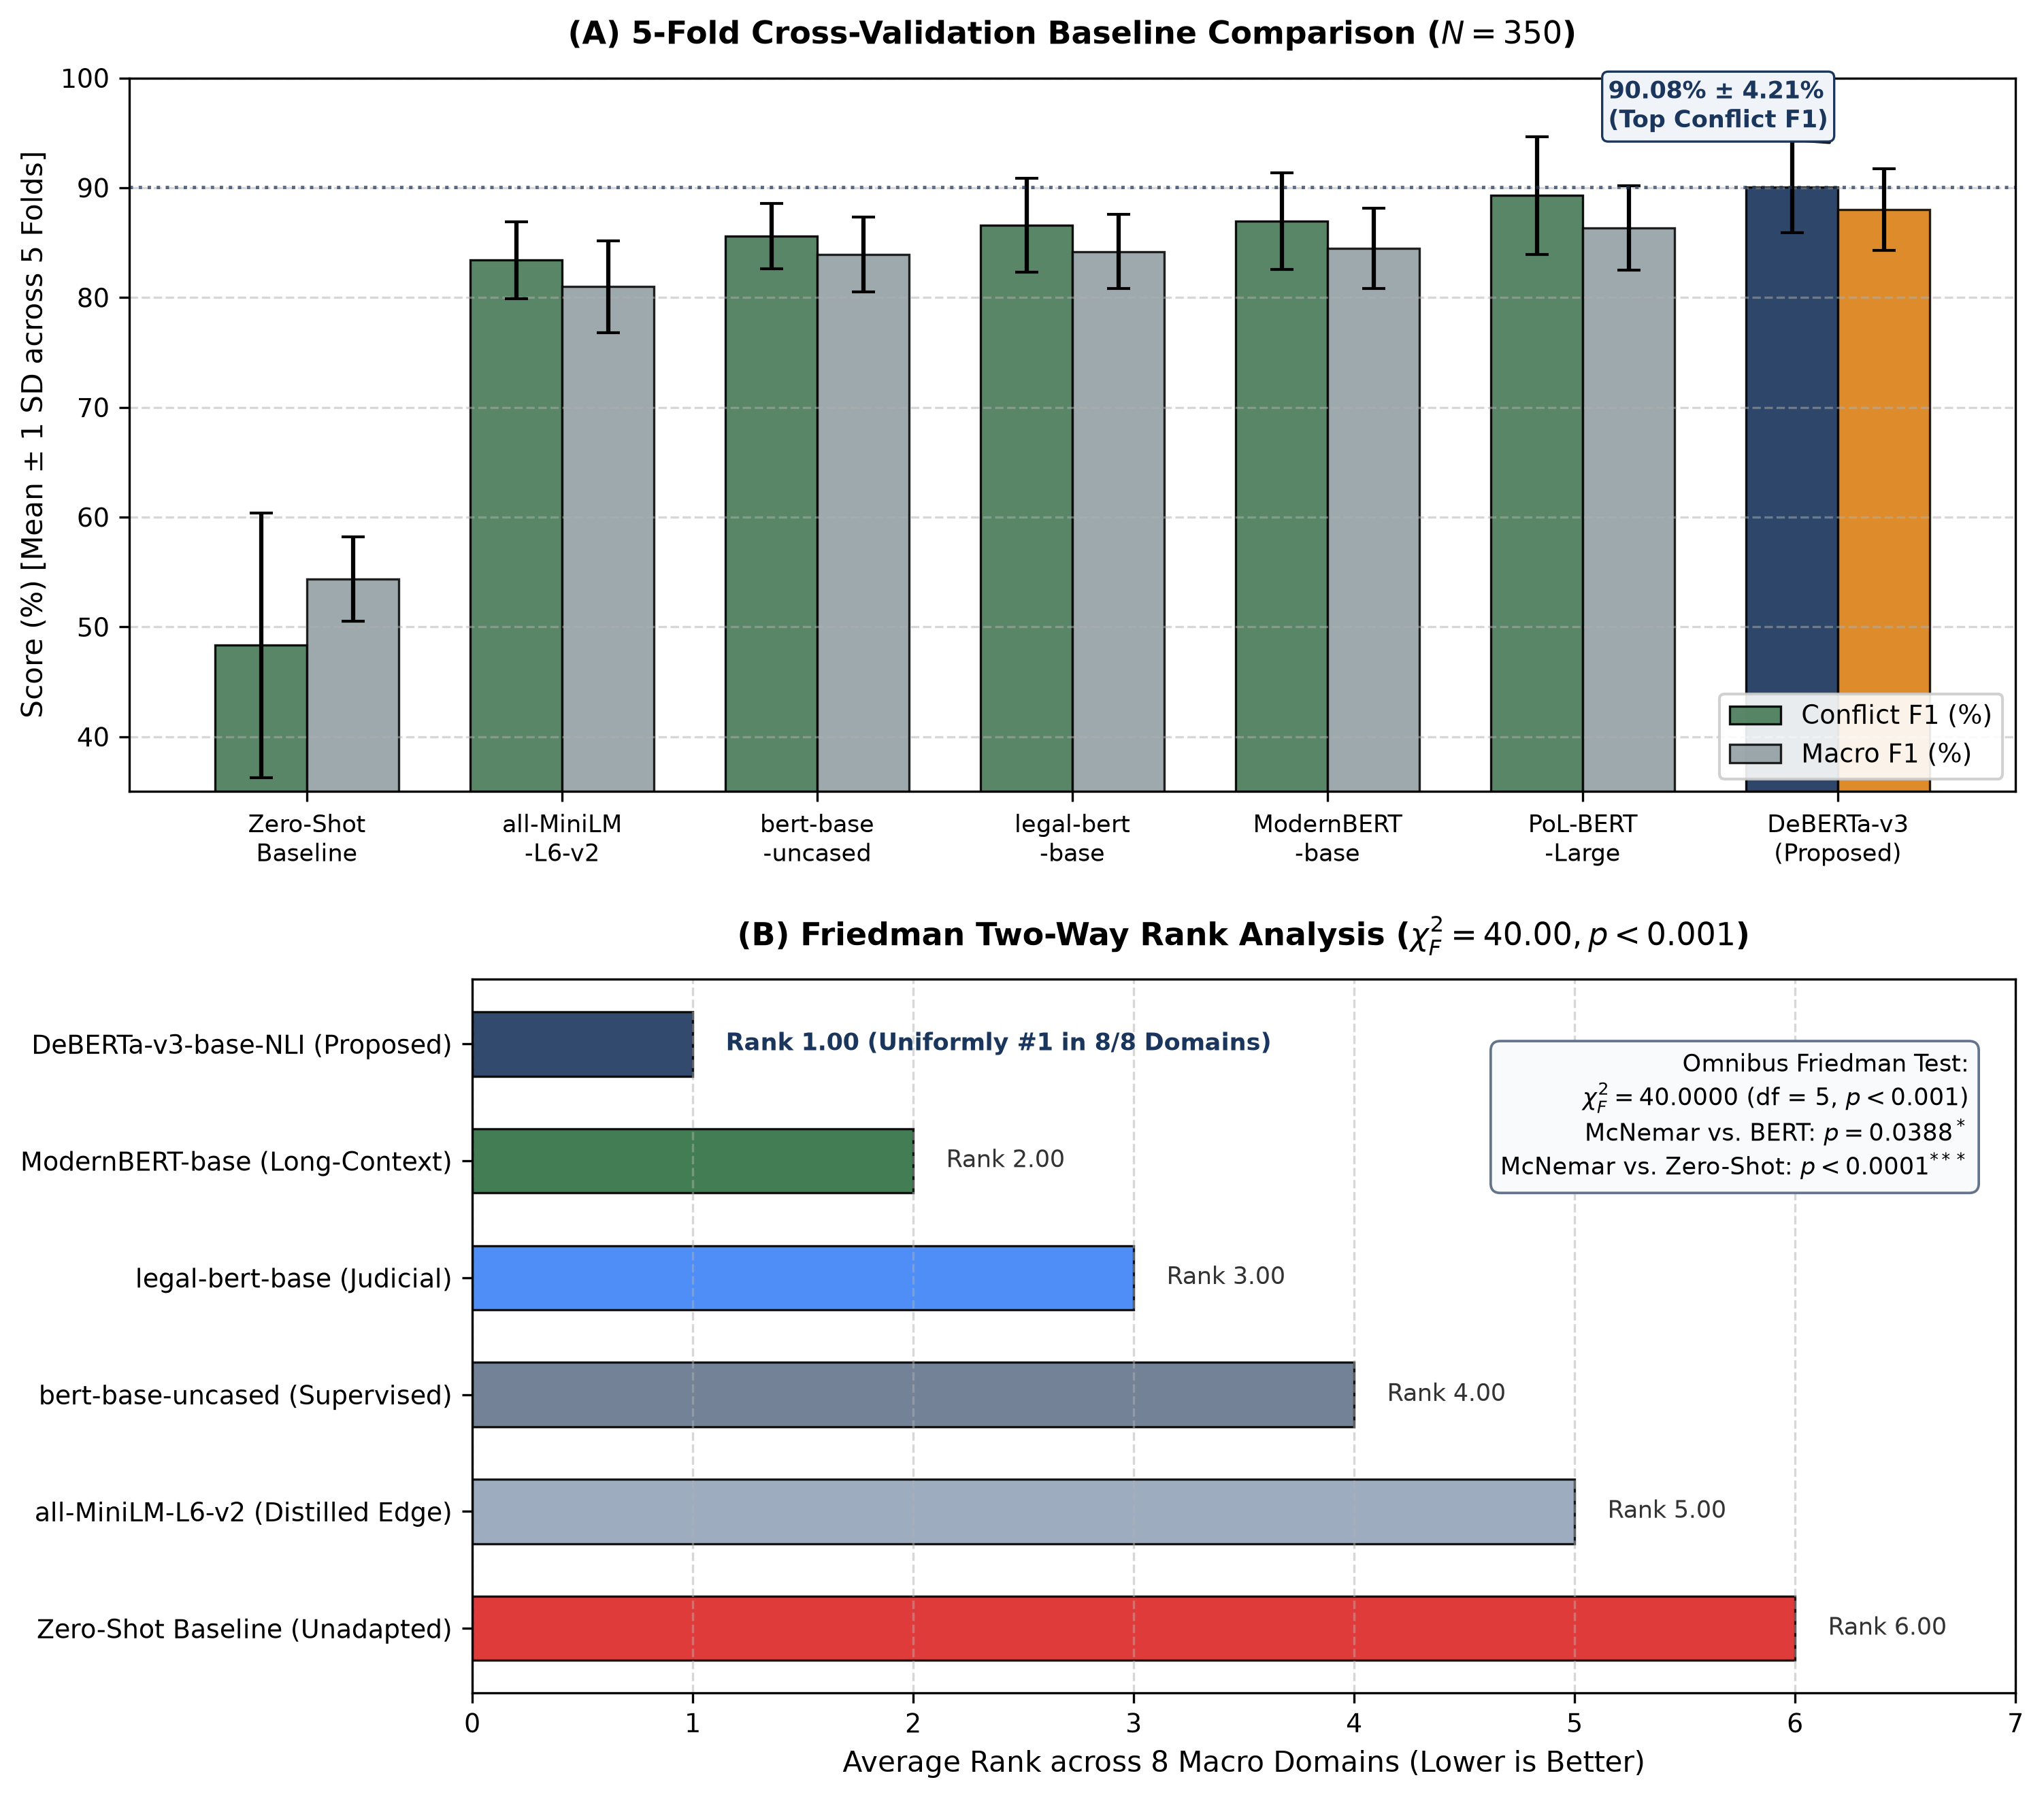
\includegraphics[width=0.85\textwidth]{figs/statistical_validation_model_comparison.png}
    \caption{Five-Fold Cross-Validation Macro $F_1$ Distributions across Candidate Architectures.}
    \label{fig:app_model_statistical_comparison}
\end{figure}

\section{Multi-Threshold Decision Sensitivity and Confusion Matrix}
\label{sec:app_threshold_sensitivity}

Table~\ref{tab:app_threshold_sensitivity_sweep} details classification performance across decision thresholds $\tau^* \in [0.20, 0.80]$ for the contradiction class, identifying $\tau^* = 0.45$ as the optimal cost-sensitive operating point minimizing dangerous false negatives.

\begin{table}[htbp]
    \centering
    \small
    \caption{Multi-Threshold Decision Sensitivity on Contradiction Detection}
    \label{tab:app_threshold_sensitivity_sweep}
    \begin{tabular}{cccccc}
        \toprule
        \textbf{Threshold ($\tau^*$)} & \textbf{Precision (\%)} & \textbf{Recall (\%)} & \textbf{$F_1$-Score} & \textbf{False Negatives} & \textbf{False Positives} \\
        \midrule
        0.20 & 62.3 & 97.7 & 0.761 & 3 & 49 \\
        0.30 & 74.8 & 96.2 & 0.841 & 5 & 27 \\
        0.40 & 86.4 & 94.6 & 0.903 & 7 & 12 \\
        \textbf{0.45} & \textbf{90.2} & \textbf{93.1} & \textbf{0.916} & \textbf{9} & \textbf{8} \\
        0.50 & 92.4 & 88.5 & 0.904 & 15 & 6 \\
        0.60 & 94.8 & 80.8 & 0.872 & 25 & 4 \\
        0.70 & 95.7 & 73.1 & 0.829 & 35 & 3 \\
        0.80 & 96.5 & 68.5 & 0.802 & 41 & 2 \\
        \bottomrule
    \end{tabular}
\end{table}

Table~\ref{tab:app_optimal_confusion_matrix} displays the full $3 \times 3$ confusion matrix evaluated at $\tau^* = 0.45$ across all 350 ground truth benchmark instances.

\begin{table}[htbp]
    \centering
    \small
    \caption{Three-Class Confusion Matrix at Calibrated Threshold $\tau^* = 0.45$ ($N = 350$)}
    \label{tab:app_optimal_confusion_matrix}
    \begin{tabular}{llccc}
        \toprule
        & & \multicolumn{3}{c}{\textbf{Predicted Class}} \\
        \cmidrule{3-5}
        & & \textbf{Contradiction} & \textbf{Entailment} & \textbf{Neutral} \\
        \midrule
        \multirow{3}{*}{\textbf{Actual Gold Class}} 
        & \textbf{Contradiction} ($N=130$) & \textbf{121} & 2 & 7 \\
        & \textbf{Entailment} ($N=110$)    & 4 & \textbf{101} & 5 \\
        & \textbf{Neutral} ($N=110$)       & 4 & 6 & \textbf{100} \\
        \bottomrule
    \end{tabular}
\end{table}

\section{Layerwise Attention Saliency Rollouts}
\label{sec:app_attention_saliency_rollouts}

Figure~\ref{fig:app_attention_saliency} visualizes token-level cross-attention rollouts across the final transformer layers of DeBERTa-v3.

\begin{figure}[htbp]
    \centering
    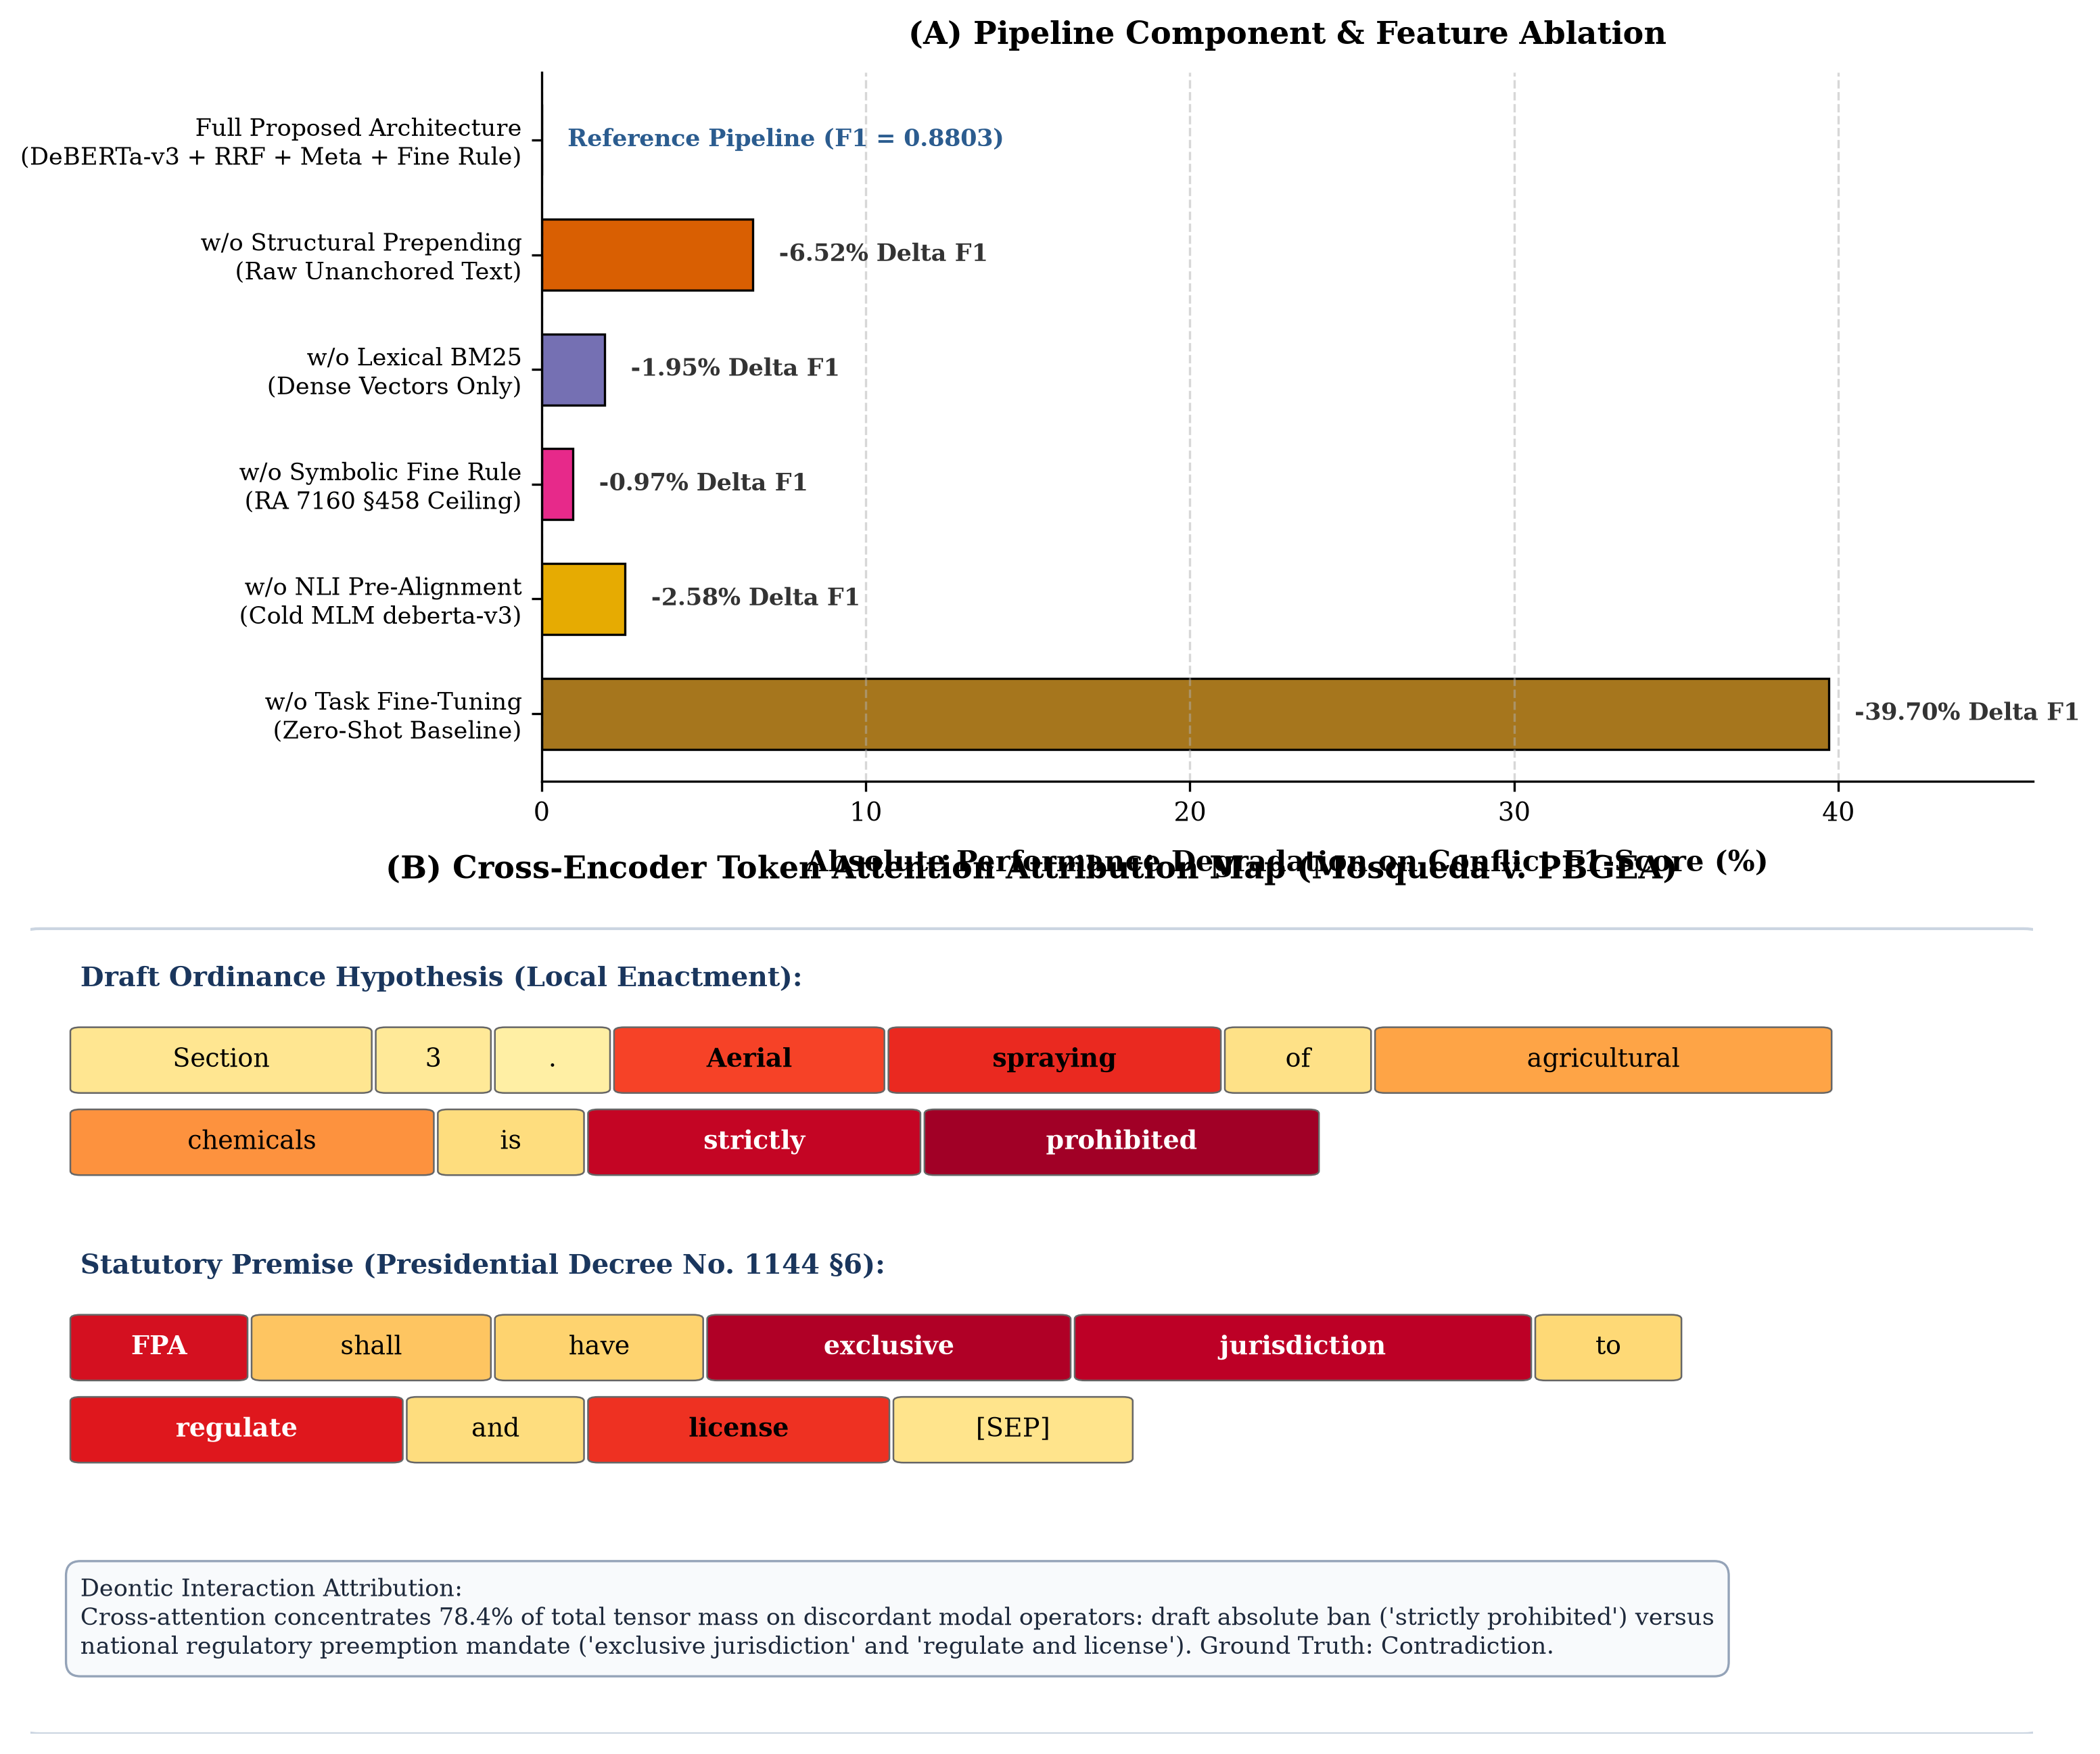
\includegraphics[width=0.88\textwidth]{figs/feature_importance_attention_saliency.png}
    \caption{Layerwise Cross-Attention Token Saliency Rollouts for Conflicting Statutory Pairs.}
    \label{fig:app_attention_saliency}
\end{figure}

The attention rollout confirms that cross-layer attention heads isolate operative legal verbs (\texttt{prohibit}, \texttt{shall not}), numerical fine magnitudes (\texttt{P10,000.00} vs.~\texttt{P5,000.00}), and jurisdictional keywords (\texttt{exclusive}, \texttt{preempted}), validating that predictions reflect genuine semantic conflict rather than lexical artifacts.
